\begin{figure}[h!]
	\centering
	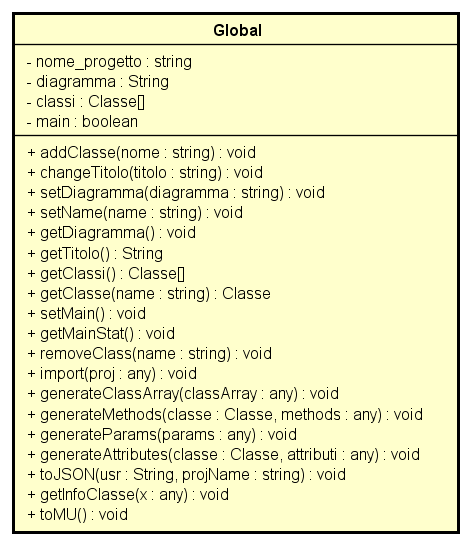
\includegraphics[scale=0.8]{res/sections/SpecificaFrontEnd/Services/Disegnetti/global.png}
	\caption{Diagramma della classe Global}
\end{figure}

\begin{itemize}
	\item \textbf{Descrizione:}\\
	
	\item \textbf{Utilizzo:}\\
	
	\item \textbf{Attributi:}
		\begin{itemize}
			\item \emph{-nome\_progetto: string}\\
			
			\item \emph{-diagramma: string}\\
			
			\item \emph{-classi: Classe[]}\\
			
			\item \emph{-main: boolean}\\
			
		\end{itemize}
	\item \textbf{Metodi:}
		\begin{itemize}
			\item \emph{+addClasse(nome: string)}\\
    		\\
    		\textbf{Parametri:}
    		\begin{itemize}
    			\item \emph{nome: string}\\
    			
    		\end{itemize}
    		\item \emph{+changeTitolo(titolo: string)}\\
    		\\
    		\textbf{Parametri:}
    		\begin{itemize}
    			\item \emph{titolo: string}\\
    			
    		\end{itemize}
    		\item \emph{+setDiagramma(diagramma: string)}\\
    		\\
    		\textbf{Parametri:}
    		\begin{itemize}
    			\item \emph{diagramma: string}\\
    			
    		\end{itemize}
    		\item \emph{+setName(name: string)}\\
    		\\
    		\textbf{Parametri:}
    		\begin{itemize}
    			\item \emph{name: string}\\
    			
    		\end{itemize}
    		\item \emph{+getDiagramma()}\\
    		
    		\item \emph{+getTitolo()}\\
    		
    		\item \emph{+getClassi()}\\
    		
    		\item \emph{+getClasse(name: string)}\\
    		\\
    		\textbf{Parametri:}
    		\begin{itemize}
    			\item \emph{name: string}\\
    			
    		\end{itemize}
    		\item \emph{+setMain()}\\
    		
    		\item \emph{+getMainStat()}\\
    		
    		\item \emph{+removeClass(name: string)}\\
    		\\
    		\textbf{Parametri:}
    		\begin{itemize}
    			\item \emph{name: string}\\
    			
    		\end{itemize}
    		\item \emph{+import(proj: any)}\\
    		\\
    		\textbf{Parametri:}
    		\begin{itemize}
    			\item \emph{proj: any}\\
    			
    		\end{itemize}
    		\item \emph{+generateClassArray(classArray: any)}\\
    		\\
    		\textbf{Parametri:}
    		\begin{itemize}
    			\item \emph{classArray: any}\\
    			
    		\end{itemize}
    		\item \emph{+generateMethods(classe: Classe, methods: any)}\\
    		\\
    		\textbf{Parametri:}
    		\begin{itemize}
    			\item \emph{classe: Classe}\\
    			
    			\item \emph{methods: any}\\
    			
    		\end{itemize}
    		\item \emph{+generateParams(params: any)}\\
    		\\
    		\textbf{Parametri:}
    		\begin{itemize}
    			\item \emph{params: any}\\
    			
    		\end{itemize}
    		\item \emph{+generateAttributes(classe: Classe, attributi: any)}\\
    		\\
    		\textbf{Parametri:}
    		\begin{itemize}
    			\item \emph{classe: Classe}\\
    			
    			\item \emph{attributi: any}\\
    			
    		\end{itemize}
    		\item \emph{+toJSON(usr: String, projName: string)}\\
    		\\
    		\textbf{Parametri:}
    		\begin{itemize}
    			\item \emph{usr: String}\\
    			
    			\item \emph{projName: string}\\
    			
    		\end{itemize}
    		\item \emph{+getInfoClasse(x: any)}\\
    		\\
    		\textbf{Parametri:}
    		\begin{itemize}
    			\item \emph{x: any}\\
    			
    		\end{itemize}
    		\item \emph{+toMU()}\\
    		
		\end{itemize}
\end{itemize}